\section{Combination of VV/VH/$\ell\ell$/$\ell\nu$}
As mentioned before, the combination of multiple signal regions would help to increase the statistics and improve the measured sensitivity.  In addition to the final state this analysis is interested in($pp\to WV \to \ell\nu qq$), there are also other analyses which are aiming for the same exotic particles. Therefore, a combination across all the possible final states of those searches was conducted to have a further improvement in the final result. The proposed scheme is to combined the diboson analyses for which the final states of VV (V=W or Z boson) decay are considered to search for the scalar boson, the HVT, and the RS graviton. And, to have a further understanding of the HVT coupling to the SM particles, the dilepton ($\ell\ell$ and $\ell\nu$) and VH ($H\to bb$) channels are also taken into the combination.
\\
\\The discriminant used in the combination is the fully reconstructed mass, $m_{WV}$, and the transverse mass, $m_{T}$ is taken when the mass could not be fully reconstructed. (like $VV\to\nu\nu\ell\ell$ or $X\to\ell\nu$).
\\
\\As discussed in the last chapter, the signal configuration was set to have a narrow resonance mass window, so the effect of interference on the cross-section is smaller than $15\%$ in the VV and VH channels. Therefore, interference is taken to be negligible. For the dilepton channel, a cut on the resonance (transverse) mass is applied to mitigate the effect. 
\subsection{Combination Strategy}
The combination scheme could be seen in Fig. \ref{Fig:Comb_scheme}, and the considered analyses with a brief event selection summary is presented in Tab. \ref{tab:signatures}.
\begin{figure}[ht]
	\centering
	\subfloat[]{\includegraphics[width=0.9\textwidth]{Chapter4/Comb_scheme.png}}
	\caption{The scheme for combination of VV, VH, and dilepton analyses with their final states.}
	\label{Fig:Comb_scheme}
\end{figure}


\begin{table}[t]
	\caption{}
	\begin{center}
		\begin{tabular}{l l c c c c c c}
			\hline
			Channel            & Diboson state & \multicolumn{4}{c}{~~~~~~Selection}       & VBF cat. & Reference \\
			&               & Leptons       & $E^{miss}_T$  & Jets   & $b$-tags &          &           \\
			\hline
			$qq qq$            & $WW/WZ/ZZ$    & 0             & veto  & 2J     & $-$      & $-$      & \cite{EXOT-2016-19} \\
			$\nu\nu qq$        & $WZ/ZZ$       & 0             & yes   & 1J     & $-$      & yes      & \cite{EXOT-2016-29} \\
			$\ell\nu qq$       & $WW/WZ$       & $1e, 1\mu$    & yes   & 2j, 1J & $-$      & yes      & \cite{EXOT-2016-28} \\
			$\ell\ell qq$      & $WZ/ZZ$       & $2e, 2\mu$    & $-$   & 2j, 1J & $-$      & yes      & \cite{EXOT-2016-29} \\
			$\ell\ell\nu\nu$   & $ZZ$          & $2e, 2\mu$    & yes   & $-$    & 0        & yes      & \cite{HIGG-2016-19} \\
			$\ell\nu\ell\nu$   & $WW$          & $1e$+$1\mu$   & yes   & $-$    & 0        & yes      & \cite{HIGG-2016-31} \\
			$\ell\nu\ell\ell$  & $WZ$          & $3e$, $2e$+$1\mu$, $1e$+$2\mu$, $3\mu$ & yes & $-$ & 0 & yes & \cite{EXOT-2016-11} \\
			$\ell\ell\ell\ell$ & $ZZ$          & $4e$, $2e$+$2\mu$, $4\mu$ & $-$ & $-$ & $-$ & yes    & \cite{HIGG-2016-19} \\
			\hline
			$qq bb$            & $WH/ZH$       & 0             & veto  & 2J     & 1, 2     & $-$      & \cite{EXOT-2016-12} \\
			$\nu\nu bb$        & $ZH$          & 0             & yes   & 2j, 1J & 1, 2     & $-$      & \cite{EXOT-2016-10} \\
			$\ell\nu bb$       & $WH$          & $1e, 1\mu$    & yes   & 2j, 1J & 1, 2     & $-$      & \cite{EXOT-2016-10} \\
			$\ell\ell bb$      & $ZH$          & $2e, 2\mu$    & veto  & 2j, 1J & 1, 2     & $-$      & \cite{EXOT-2016-10} \\
			\hline
			$\ell\nu$          & $-$           & $1e, 1\mu$    & yes   & $-$    & $-$      & $-$      & \cite{EXOT-2016-06} \\
			$\ell\ell$         & $-$           & $2e, 2\mu$    & $-$   & $-$    & $-$      & $-$      & \cite{EXOT-2016-05} \\
			\hline
		\end{tabular}
		\label{tab:signatures}
	\end{center}
\end{table}


\noindent
\\With the number of involved analyses, the likelihood construction of all the final state would be too complicated, so the procedure was conducted step by step. It started from the same medium states of WW, WZ, or ZZ bosons with their fermionic final states, and then, they are integrated into the VV combination. At this stage, the statistic interpretations on RS graviton and NWA scalar boson are completed. Following by that, the VV channels are combined together with VH and dilepton channels to set the limit on mass of W' and Z' bosons as well as the coupling strength between the HVT and SM particles.  
\\
\\{\bf Orthogonality }
\\
\\Within VV and VH channels, the category orthogonality was kept by the cuts on lepton number, $E^{miss}_T$, and b-jet numbers. However, to have the selection on the boson decayed jets, the mass windows were overlapped between W/Z and Higgs bosons, so some events went into both VV and VH signal regions. Tab. \ref{Tab:VVVH_masswindow} shows the mass windows used in the hadronically decayed bosons. In this case, the events are given higher priority to go into the VV category and get removed from the VH channels, if the selected dijet system has the mass in the overlapped region. With the comparison to the original event selection, the expected sensitivity doesn't have significant change ($<10\%$) which could be seen in Fig. \ref{Fig:limits_Hbb}. 
\begin{table}
	\caption{The mass windows for the selection on hadronically decayed bosons in VV and VH events}
	\label{Tab:VVVH_masswindow}
	\begin{tabular}{c|c|c|c|c}
		\hline
		channel                                    & Jet Topo  & W       &    Z     &  H \\
		\hline
		\hline
		\multirow{ 2}{*}{$qqqq$}                   & resolved  & - & - &  - \\
		\cline{2-5}
                                                   & merged    & [65,95] & [76,106] &  - \\
		\hline
		\multirow{ 2}{*}{$\ell\ell qq$}            & resolved  & [62,97] & [70,105] &  - \\
		\cline{2-5}
                                                   & merged    & [65,95] & [76,106] &  - \\
		\hline 
		\multirow{ 2}{*}{$\ell\nu qq$}             & resolved  & [66,94] & [82,106] &  - \\
		\cline{2-5}
                                                   & merged    & [64,104](LP) & [69,114](LP) &  - \\
		\hline
		\multirow{ 2}{*}{$\nu\nu qq$}              & resolved  & - & - &  - \\
		\cline{2-5}
                                                   & merged    & [65,95] & [76,106] &  - \\
		\hline 
		\multirow{ 2}{*}{$qqbb$}                   & resolved  & - & - &  - \\
		\cline{2-5}
                                                   & merged    & - & [70,110] (HP) &  [75,145] \\
		\hline 
		\multirow{ 2}{*}{$\ell\nu bb$/$\nu\nu bb$} & resolved  & \multicolumn{3}{c}{[110,140]} \\
		\cline{2-5}
                                                   & merged    & \multicolumn{3}{c}{[75,145]} \\
	    \hline
		\multirow{ 2}{*}{$\ell\ell bb$}            & resolved  & \multicolumn{3}{c}{[100,145]} \\
        \cline{2-5}
                                                   & merged    & \multicolumn{3}{c}{[75,145]} \\
        \hline
	\end{tabular}
\end{table} 
\begin{figure}[ht]
	\centering
	\subfloat[]{\includegraphics[width=0.34\textwidth]{Chapter4/vvbb_limit.png}}
	\subfloat[]{\includegraphics[width=0.34\textwidth]{Chapter4/lvbb_limit.png}}	\subfloat[]{\includegraphics[width=0.34\textwidth]{Chapter4/llbb_limit.png}}
	\caption{The change in expected limits in the VH channels for (a)$VH\to\nu\nu bb$ (b)$VH\to\ell\nu bb$ and (c) $VH\to\ell\ell bb$ }
	\label{Fig:limits_Hbb}
\end{figure}
\noindent
\\
\\{\bf Nuisance Parameter Correlation}
\\
\\For each individual analysis, more than 100 nuisance parameters are considered. Some of them are commonly applied across the analyses, but there are also the ones which only made the contribution to the dedicated analyses. The following is the list of nuisance parameters which are decorrelated from the other analyses:
\begin{itemize}
	\item[] {\bf Jet Uncertainties}: The measurement of jets actually have 81 sources of uncertainties, but most of analyses just deploy the simplified schemes for which the 81 sources are combined into 21 or 3 uncertainties. For the analyses using different simplified uncertainty schemes, their jet uncertainties are decorrelated ($VV\to\ell\nu\ell\ell\&\ell\ell\nu\nu$)
	\item[] {\bf Electron ID Uncertainty}: The  $VV\to\ell\nu\ell\nu$ analysis has deployed different identification working points in the electron selection, so the related uncertainty is decorrelated. 
	\item[] {\bf Signal and Background Modelling Uncertainties}: The scale factors for the SM background in the likelihood reconstructions are decorrelated as they have different kinematic properties for varied final states. Furthermore, the uncertainties arising from the data-driven estimation are also decorrelated. As the ISR/FSR effect was not considered in the fully leptonically decayed channels, they are decorrelated as well.  
\end{itemize}
\subsection{Result}
The combination is aiming for two kind of results: the limit on the mass of exotic partices (NWA scalar boson, HVT W' and Z' bosons, and RS gravtion), and the limit on the coupling strength between the HVT and SM particles. The first result will follow the asymptotic methodology which was discuss in Sec.\ref{Sec:lvqq_result} with a cross-check from the toy model\footnote{as running the toy model is computationally expensive, it it only performed on the mass points of 1, 2, 3, 4, and 5 TeV}, and , for the second result, a similar likelihood would be constructed by the parameter of interest would be the coupling constant, $\vec{g}$, instead of the signal strength, $\mu$. The detail will be coming later. 
\\
\\{\bf Mass Limits}
\\
\\The cross-section limits are set with the ggF/DY and VBF productions respective. For the VBF category, not all analyses have this channel, but they are still combined to provide the upper limit, and the results are shown in Fig.~\ref{Fig:limit_VBF_comb}. Here, a new benchmark for the HVT model is applied with $g_{H}=1$ and $g_{f}=0$, and this means the production of W' and Z' bosons could only be via VBF. With model c, the sensitivity is set as the inclusive (W' + Z' bosons) cross-section upper limit ratio between the expectation (observation) and theory. With respect to the single channel analysis presented before, the mass limit has seen a significant improvement from $1.2~TeV$($3~TeV$) to $2.2~TeV$($4.5~TeV$) for the RS graviton (HVT boson) interpretation.   
\begin{figure}[ht]
	\centering
	\subfloat[]{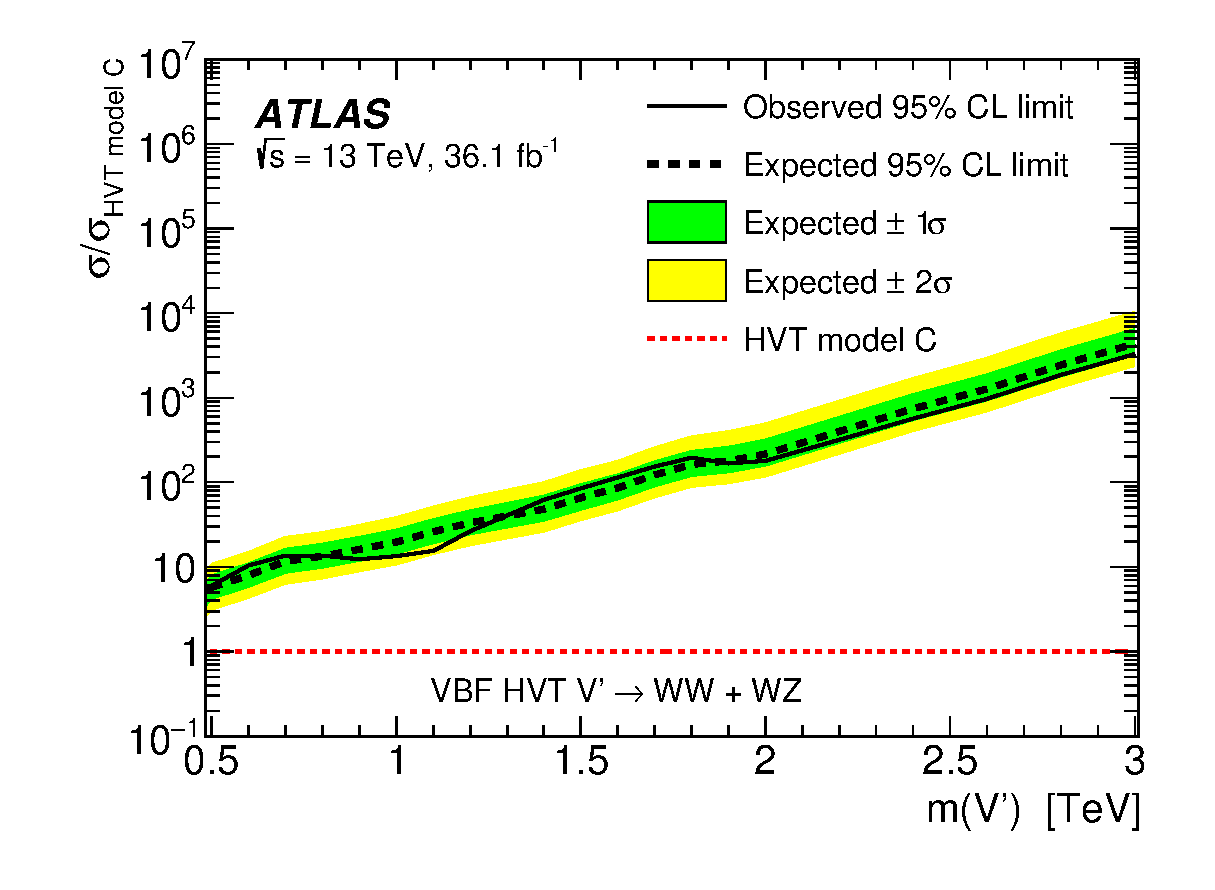
\includegraphics[width=0.5\textwidth]{Chapter4/VBFWWWZHVT_COMB.eps}}
	\subfloat[]{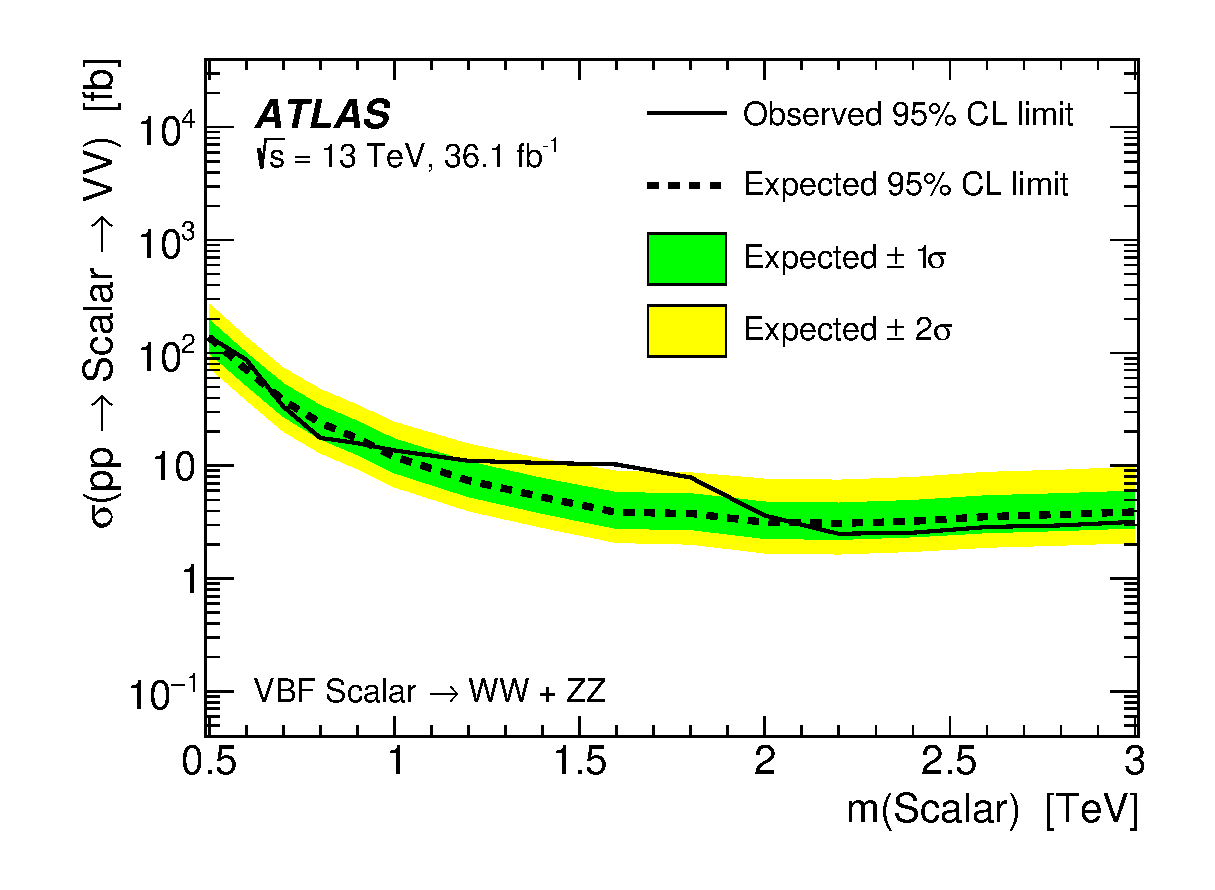
\includegraphics[width=0.5\textwidth]{Chapter4/VBFWWZZNWA_COMB.eps}}
	\caption{The cross-section upper limit for (a) the HVT model boson (as a ratio to the theoretical one) (b) and the NWA scalar boson }
	\label{Fig:limit_VBF_comb}
\end{figure}
\noindent
\\
\\For the ggF result, the VV channel is combined with VH and dilepton channels for the HVT interpretation, while the limits on models of RS graviton and NWA scalar boson are only set with the VV channel. The HVT interpretation is shown in Fig.~\ref{Fig:limit_GGFHVT_comb} as the ratio to the theoretically predicted cross-section. And, The limits on RS graviton and NWA scalar bosons are in Fig.~\ref{Fig:limit_GGF_comb}, while Fig.~\ref{Fig:limit_GGFHVTV_compare} is presenting the comparison of the sensitivities from the VV+VH and dilepton channels. 
\begin{figure}[ht]
	\centering
	\subfloat[]{\includegraphics[width=0.5\textwidth]{Chapter4/GGFALLHVTW_COMB.eps}}
	\subfloat[]{\includegraphics[width=0.5\textwidth]{Chapter4/GGFALLHVTZ_COMB.eps}}
	\caption{The cross-section upper limit ratio to the HVT model theoretical prediction for (a) the W' boson (b) the Z' boson }
	\label{Fig:limit_GGFHVT_comb}
\end{figure}
\begin{figure}[ht]
	\centering
	\subfloat[]{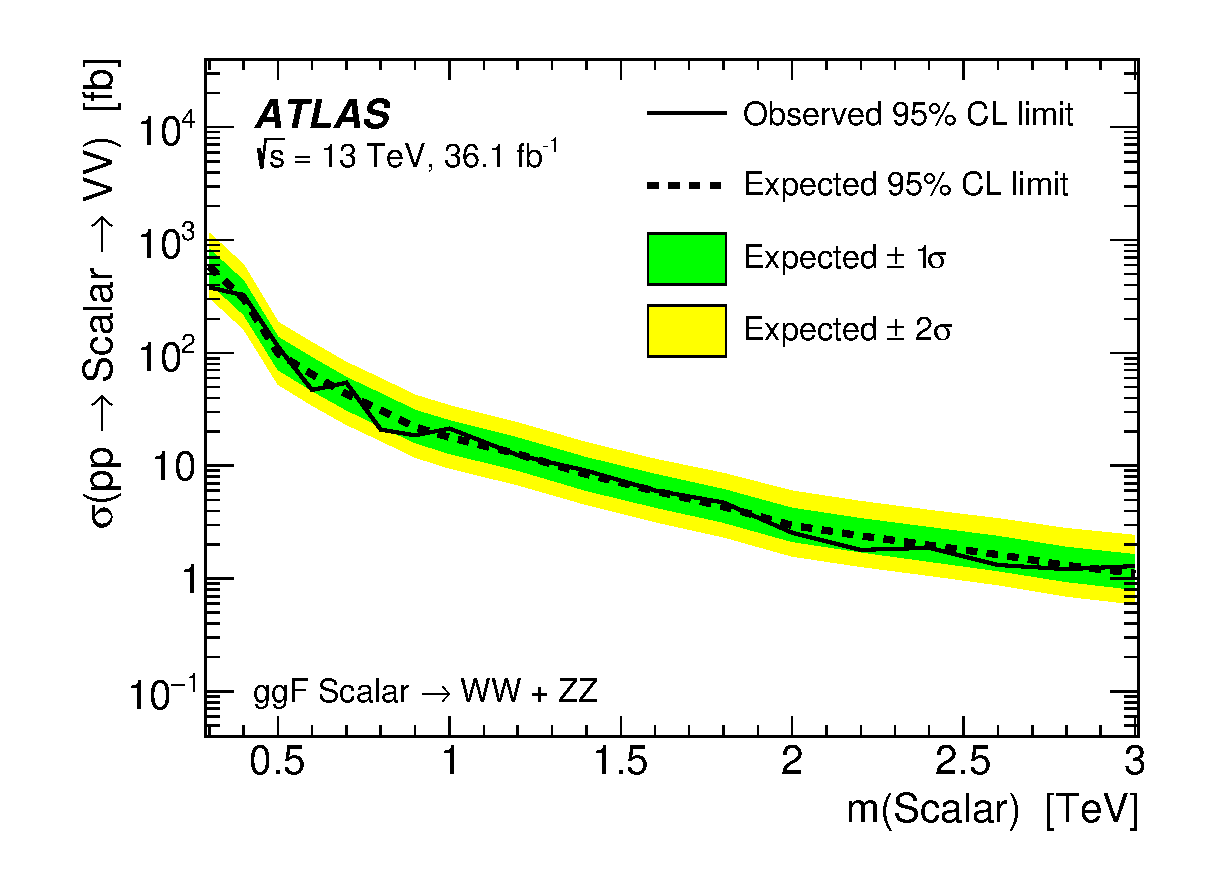
\includegraphics[width=0.5\textwidth]{Chapter4/GGFWWZZNWA_COMB.eps}}
	\subfloat[]{\includegraphics[width=0.5\textwidth]{Chapter4/GGFWWZZRSG_COMB.eps}}
	\caption{The cross-section upper limit ratio to the (a) NWA scalar boson (b) RS graviton}
	\label{Fig:limit_GGF_comb}
\end{figure}
\begin{figure}[ht]
	\centering
    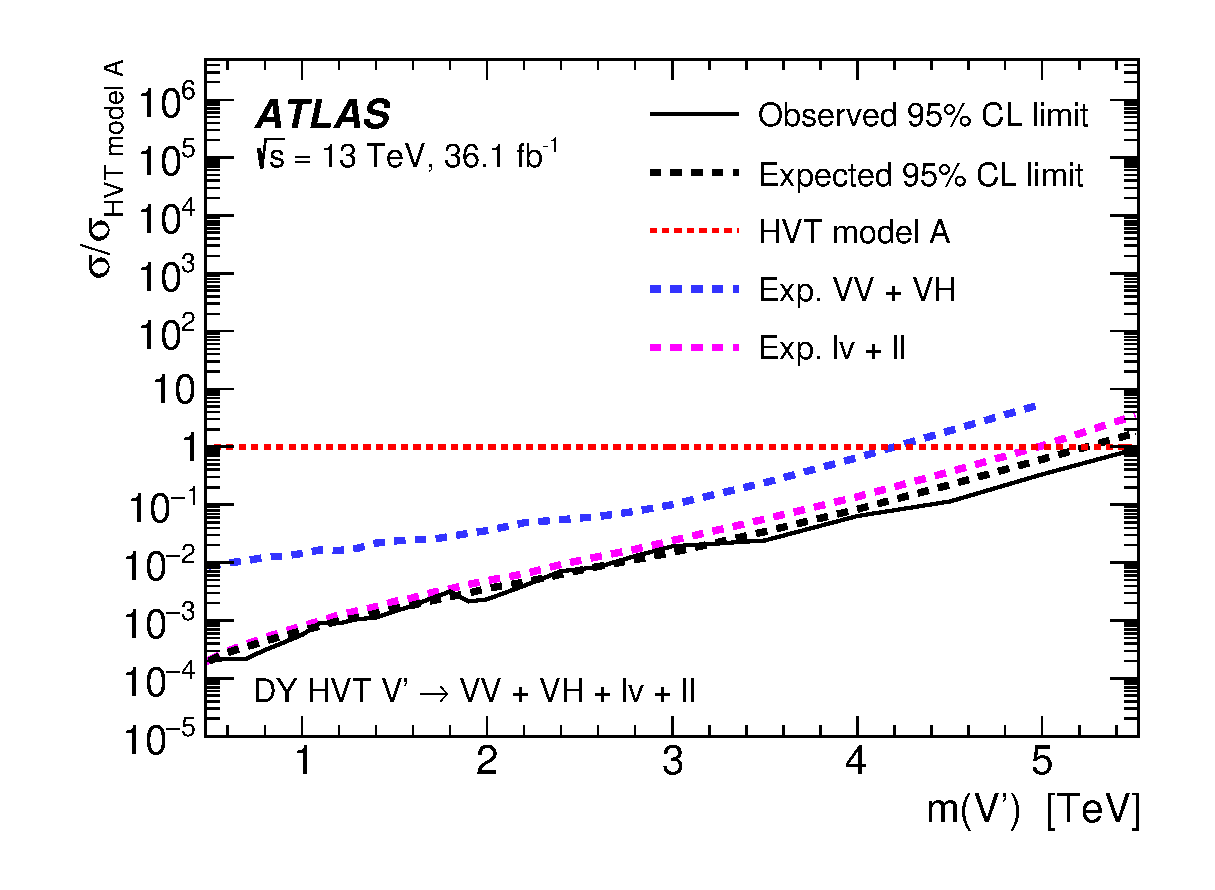
\includegraphics[width=0.5\textwidth]{Chapter4/GGFALLHVTV_compare.eps}
    \caption{The comparison on the limits on the HVT V' bosons set by different channels}
	\label{Fig:limit_GGFHVTV_compare}
\end{figure}
\noindent
\\
\\{\bf Coupling Limits}
\\
\\The limits of the HVT couplings are set on a two-dimensional plane with which two pairs of parameters are used:
\begin{itemize}
  \item[] {\bf $g_{H}$ and $g_{f}$}: they are corresponding to the couplings to the SM bosons (W, Z, and H) and fermions. For the simplicity, the fermionic coupling is set equal between quarks and leptons. 
  \item[] {\bf $g_{l}$ and $g_{q}$}: they are corresponding to the couplings to the leptons and quarks with the coupling to SM bosons set at 0.56 (model A).
\end{itemize}
\noindent
\\For the estimation of the couplings, the same method in Sec.\ref{Sec:lvqq_result} is applied with the profile likelihood and asymptotic formulae, but the likelihood is constructed with the coupling strengths:
\begin{equation}
\lambda(\vec{\mathcal{G}}) = \frac{\mathcal{L}(\vec{\mathcal{G}},\hat{\hat{\theta}})}{\mathcal{L}(\hat{\vec{\mathcal{G}}},\hat{\theta})}
\end{equation}
Then, the event yields (signal strength) would be parametrized in terms of the couplings, and the following procedure be to set the exclusion limit at the $95\%$ confidence level .
\\
\\The final results are shown in Fig.~\ref{Fig:limit_coupling} on which the region outside dotted lines are excluded, and the results from the electroweak precision measurement \cite{delAguila:2010mx} are also overlaid as the coloured exclusion region which has combined the following experiments:
\begin{itemize}
	\item Z mass pole measurements from LEP\cite{delAguila:2010mx}
	\item LEP2 measurements provided in the last joint paper by the ALEPH, DELPHI, L3, and OPAL Collaborations\cite{Schael:2013ita}
	\item Measurements from low-energy experiments, CKM unitarity and $\alpha_{s}$\cite{Olive_2016}
	\item World average for the top-quark mass measurements from the ATLAS, CMS, CDF, and D0 Collaborations\cite{ATLAS:2014wva}
	\item World average for the Higgs boson mass measurements with Run 1 data from the ATLAS and CMS Collaborations (the cross-section measurement is not included)\cite{Aad:2015zhl}
\end{itemize}   
\begin{figure}[ht]
	\centering
	\subfloat[]{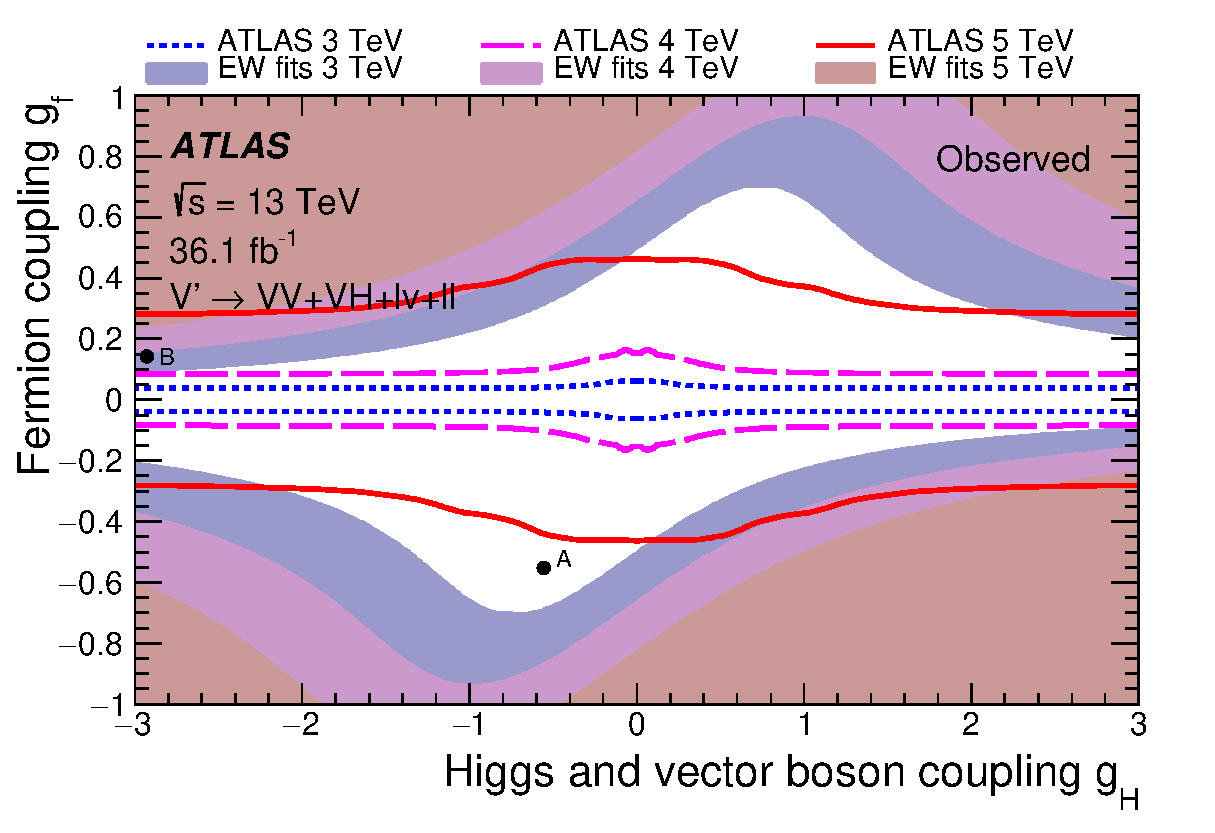
\includegraphics[width=0.5\textwidth]{Chapter4/Coupling_hf_all.eps}}
	\subfloat[]{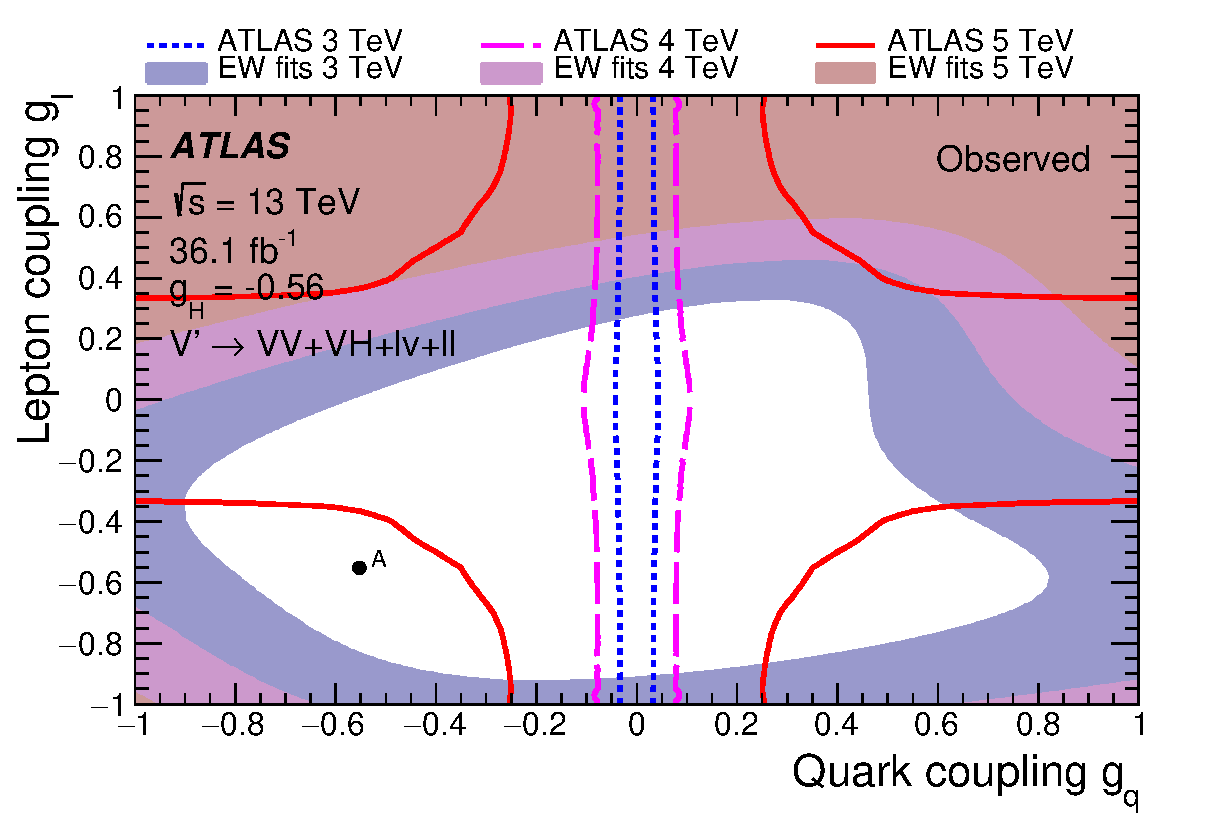
\includegraphics[width=0.5\textwidth]{Chapter4/Coupling_lg_all.eps}}
	\caption{The limits on coupling strength from the full combination with (a) {$g_H, g_f$} and (b) {$g_l, g_q$} planes }
	\label{Fig:limit_coupling}
\end{figure}
\noindent
\\
\\It could be seen that the combination of exotic particle searches has presented the exclusion that the electroweak measurements didn't have the sensitivity. With the low mass HVT boson assumptions, both of the two benchmark models are also excluded by the coupling strength interpretation.
\section{Summary}
In the search for new particles with diboson resonance, the single final state of $WV\to\ell\nu qq$ is chosen to investigate two production modes, ggF/DY (indistinguishable) and VBF, along two jet topologies. The background estimation was performed with the Monte Carlo simulation for the Standard Model process like W+jets and $t\bar{t}$ interactions and the Fake Factor method for the multijet events. After the comparison between background estimation and data with a statistic interpretation, the discovery significance didn't confirm the existence of any unknown particle. Therefore, the limits are set via the asymptotic method on the particle mass based the present analysis sensitivity. 
\\
\\For the further enhancement on the sensitivity to new physics, the $\ell\nu qq$ result was combined with the other diboson and dilepton final states. However, there is still no evident existence of the new particles. The limits on the particle mass and their coupling to the SM particle are then set giving an improved constraint on the phase space for the new particle searches.  